% ---------------------------------------------------------------------
% --- Arquivo principal e os demais serao os dos capitulos.
% --- EXPRESSOES ENTRE <> DEVERAO SER COMPLETADAS COM A INFORMACAO ESPECIFICA DO TRABALHO 
% ---------------------------------------------------------------------

\documentclass[ruledheader]{abnt_UFF}
    
%---pacotes para hiphenizacao e acentuacao em portugues
\usepackage[brazil]{babel}
\usepackage[utf8]{inputenc}
\usepackage[T1]{fontenc}



%--- pacote para figuras
\usepackage{epsf}
\usepackage[dvips]{epsfig,graphicx}
\usepackage{subfigure}


%--- pacote de simbolos
\usepackage{latexsym}
\usepackage{textcomp}

%--- simbolos matematicos
\usepackage{amsmath}
\usepackage{amssymb}

%--- pacote para gerar pseudo-codigo
\usepackage{algorithm}
\usepackage{algorithmic}
\floatname{algorithm}{Algoritmo}

%--- outros pacotes
\usepackage{url}
\usepackage{longtable}
\usepackage{lscape}


%Tabela Colorida
\usepackage{colortbl}


\usepackage{multicol}
\usepackage{multirow}
\usepackage{rotating}


\hyphenation{
a-de-qua-da-men-te 
di-men-sio-na-men-to 
}

%---------usando tipo de fonte padrao
\renewcommand{\ABNTchapterfont}{\bfseries\fontfamily{cmr}\fontseries{b}\selectfont}
\renewcommand{\ABNTsectionfont}{\bfseries\fontfamily{cmr}}


% --- -----------------------------------------------------------------
% --- Documento Principal.
% --- -----------------------------------------------------------------
% \usepackage[pdftex]{hyperref}
% \hypersetup{colorlinks, sitecolor=black, pdftex}
\begin{document}

% --- -----------------------------------------------------------------
% --- Titulo, abstract, dedicatorias e agradecimentos.
% --- Indice geral, lista de figuras e tabelas.
% --- -----------------------------------------------------------------
% --- -----------------------------------------------------------------
% --- Elementos usados na Capa e na Folha de Rosto.
% --- EXPRESSOES ENTRE <> DEVERAO SER COMPLETADAS COM A INFORMACAO ESPECIFICA DO TRABALHO
% --- E OS SIMBOLOS <> DEVEM SER RETIRADOS 
% --- -----------------------------------------------------------------
\autor{LUCAS DE SOUZA TITO} % deve ser escrito em maiusculo

\titulo{Apoio Computacional na Predição Epidemiológica e Filodinâmica de Doenças Infecciosas Emergentes}

\instituicao{UNIVERSIDADE FEDERAL FLUMINENSE}

\orientador{DANIEL CARDOSO MORAES DE OLIVEIRA}

\coorientador{KARY ANN DEL CARMEN OCAÑA GAUTHEROT} % se nao existir co-orientador apague essa linha

\local{NITER\'{O}I}

\data{2019} % ano da defesa

\comentario{Dissertação de Mestrado apresentada ao Programa de P\'{o}s-Gradua\c{c}\~{a}o em Computa\c{c}\~{a}o da \mbox{Universidade} Federal Fluminense como requisito parcial para a obten\c{c}\~{a}o do Grau de \mbox{Mestre em Computa\c{c}\~{a}o}. \'{A}rea de concentra\c{c}\~{a}o: \mbox{Engenharia de Sistemas e Informação}} %preencha com a sua area de concentracao


% --- -----------------------------------------------------------------
% --- Capa. (Capa externa, aquela com as letrinhas douradas)(Obrigatorio)
% --- ----------------------------------------------------------------
\capa

% --- -----------------------------------------------------------------
% --- Folha de rosto. (Obrigatorio)
% --- ----------------------------------------------------------------
\folhaderosto


\pagestyle{ruledheader}
\setcounter{page}{1}
\pagenumbering{roman}

% --- -----------------------------------------------------------------
% --- Termo de aprovacao. (Obrigatorio)
% --- ----------------------------------------------------------------
\cleardoublepage
\thispagestyle{empty}

\vspace{-60mm}

\begin{center}
   {\large LUCAS DE SOUZA TITO}\\
   \vspace{7mm}

Apoio Computacional na Predição Epidemiológica e Filodinâmica de Doenças Infecciosas Emergentes    \\
  \vspace{10mm}
\end{center}

\noindent
\begin{flushright}
\begin{minipage}[t]{8cm}

Dissertação de Mestrado apresentada ao Programa de P\'{o}s-Gradua\c{c}\~{a}o em Computa\c{c}\~{a}o da Universidade Federal Fluminense como requisito parcial para a obten\c{c}\~{a}o do \mbox{Grau} de Mestre em Computa\c{c}\~{a}o. \'{A}rea de concentra\c{c}\~{a}o: \mbox{Engenharia de Sistemas e Informação} %preencha com a sua area de concentracao

\end{minipage}
\end{flushright}
\vspace{1.0 cm}
\noindent
Aprovada em <MES> de <ANO>. \\
\begin{flushright}
  \parbox{11cm}
  {
  \begin{center}
  BANCA EXAMINADORA \\
  \vspace{6mm}
  \rule{11cm}{.1mm} \\
    Prof. Daniel Cardoso Moraes de Oliveira - Orientador, IC/UFF \\
    \vspace{6mm}
  \rule{11cm}{.1mm} \\
    Kary Ann del Carmen Ocana Gautherot, LNCC\\
    \vspace{6mm}
  \rule{11cm}{.1mm} \\
    Prof. <NOME DO AVALIADOR>, <INSTITUI\c{C}\~AO>\\
  \vspace{4mm}
  \rule{11cm}{.1mm} \\
    Prof. <NOME DO AVALIADOR>, <INSTITUI\c{C}\~AO>\\
    \vspace{6mm}
  \rule{11cm}{.1mm} \\
    Prof. <NOME DO AVALIADOR>, <INSTITUI\c{C}\~AO>\\
  \vspace{6mm}
  \end{center}
  }
\end{flushright}
\begin{center}
  \vspace{4mm}
  Niter\'{o}i \\
  %\vspace{6mm}
  2019

\end{center}

% --- -----------------------------------------------------------------
% --- Dedicatoria.(Opcional)
% --- -----------------------------------------------------------------
\cleardoublepage
\thispagestyle{empty}
\vspace*{200mm}

\begin{flushright}
{\em 
Dedicatória(s): Dedico este trabalho a Deus, minha mãe Patrícia Andréa e ao meu irmão Caio Vinícius que são os pilares da minha vida e cujo amor funcionou como força motriz na realização e conclusão desta dissertação.
}
\end{flushright}
\newpage


% --- -----------------------------------------------------------------
% --- Agradecimentos.(Opcional)
% --- -----------------------------------------------------------------
\pretextualchapter{Agradecimentos}
\hspace{5mm}
Gostaria de agradecer aos meus melhores amigos: Marcelo D'Almeida, Kelly Tavares, Nathan Gerhard, Guilherme Alves, Victor Olimpio, Sandra Fratane, Felipe Santiago, Alexandre Estebanez, Felipe Lugão Eccard, Rodrigo Rodovalho e André Alvarado por me apoiarem e ajudarem a resolver problemas em código, debugar, configurar ambiente, revisar este trabalho, me ouvirem reclamar da vida ou me obrigarem a sair pra relaxar e não perder a cabeça (não necessariamente nessa ordem); ao melhor professor do IC/UFF, meu orientador Daniel de Oliveira, por todos os conselhos, toda a ajuda e principalmente, por toda a paciência comigo quando eu o perturbava; e minha gestora Paula Mian por toda a compreensão e flexibilidade nos meus horários tornando viável a continuidade do mestrado em paralelo a minhas atividades na Muxi Tecnologia S.A o qual sou grato pelo tempo de empresa e todo o aprendizado adquirido; ao meu avô Florentino mangueira, por compartilhar comigo suas histórias, suas experiências de vida e por servir como um grande exemplo de perseverança; ao Roberto Carlos Melo, por ajudar na construção do meu caráter e me auxiliar em diferentes momentos do meu cotidiano; a todos os meus professores e à todas as minhas professoras, do jardim até a pós-graduação, que passaram parte dos seus conhecimentos para mim. Também aos meus colegas e familiares que sempre foram presentes apesar da distância. Além daqueles que encontrei diariamente ao decorrer da minha vida e cujo nome não sei ou esqueci (faxineiros, cobradores de ônibus, vendedores ambulantes, porteiros e demais), pessoas que alegraram meu dia, sendo educados e respeitosos, oferecendo alguma ajuda por mais singela que pareça.

% --- -----------------------------------------------------------------
% --- Resumo em portugues.(Obrigatorio)
% --- -----------------------------------------------------------------
\begin{resumo}

Este trabalho apresenta o uso de técnicas e ferramentas de data science e e-science em tarefas de pré-processamento, integração, consulta e visualização dos dados como apoio computacional para a predição epidemiológica e filodinâmica de doenças infecciosas emergentes como Zika. A principal base de dados utilizada foi extraída do Sistema Gerenciador de Ambiente Laboratorial (GAL), que quando integrada a outras informações permitiu a obtenção de resultados interessantes, dentre eles a taxa positiva de infecção por metodologia e por material coletado. Essas informações podem ser usadas para o aprimoramento da gestão da saúde pública, direcionando recursos e tornando o processo de diagnóstico de doenças mais efetivo.

{\hspace{-8mm} \bf{Palavras-chave}}: Palavras representativas do conteúdo do trabalho, isto é, palavras-chave e/ou descritores, conforme a ABNT NBR 6028 (ABNT, 2005).

\end{resumo}

% --- -----------------------------------------------------------------
% --- Resumo em lingua estrangeira.(Obrigatorio)
% --- -----------------------------------------------------------------
\begin{abstract}

This work introduces the use of data science and e-science tools and techniques in preprocessing, integrating, querying and visualizing data as computational support for the epidemiological and philodynamic prediction of emerging infectious diseases such as Zika. The main database has been extracted from the Laboratory Environment Management System (GAL), which has been integrated with other information, allowing to obtain interesting results, among them the positive rate of infection by methodology and material collected. This information can be used to improve public health management by directing resources and making the disease diagnosis process more effective.

{\hspace{-8mm} \bf{Keywords}}: Palavras representativas do conteúdo do trabalho, isto é, palavras-chave e/ou descritores, na língua (ABNT, 2005).

\end{abstract}

% --- -----------------------------------------------------------------
% --- Lista de figuras.(Opcional)
% --- -----------------------------------------------------------------
%\cleardoublepage
\listoffigures


% --- -----------------------------------------------------------------
% --- Lista de tabelas.(Opcional)
% --- -----------------------------------------------------------------
\cleardoublepage
%\label{pag:last_page_introduction}
\listoftables
\cleardoublepage

% --- -----------------------------------------------------------------
% --- Lista de abreviatura.(Opcional)
%Elemento opcional, que consiste na relacao alfabetica das abreviaturas e siglas utilizadas no texto, seguidas das %palavras ou expressoes correspondentes grafadas por extenso. Recomenda-se a elaboracao de lista propria para cada %tipo (ABNT, 2005).
% --- ----------------------------------------------------------------
\cleardoublepage
\pretextualchapter{Lista de Abreviaturas e Siglas}
\begin{tabular}{lcl}
<ABREVIATURA> & : & <SIGNIFICADO>;\\
<ABREVIATURA> & : & <SIGNIFICADO>;\\
<ABREVIATURA> & : & <SIGNIFICADO>;\\
\end{tabular}
% --- -----------------------------------------------------------------
% --- Sumario.(Obrigatorio)
% --- -----------------------------------------------------------------
\pagestyle{ruledheader}
\tableofcontents




% --- -----------------------------------------------------------------
% --- Insercao dos capitulos.
% --- -----------------------------------------------------------------
\pagestyle{ruledheader}
\setcounter{page}{1}
\pagenumbering{arabic}
\chapter{T\'itulo do primeiro cap\'itulo} \label{cap:cap1}

Este \'e o primeiro cap\'itulo. 

\section{Introdu\c{c}\~ao}\label{sec:intro}

Este \'e a introdu\c{c}\~ao do primeiro cap\'itulo. 

Exemplo de Figura: Ver Figura~\ref{fig:exefig}.

\begin{figure}[!ht]
\centering

\includegraphics[width=0.3\linewidth]{figuras/exefig.eps}
\caption{Exemplo de figura}
\label{fig:exefig}
\end{figure}

Este \'e o primeiro cap\'itulo. 

Exemplo de refer\^encias~\cite{tese2011, confinter2011, confnac2011, rev2011, site2011}.

Este \'e o primeiro cap\'itulo. 

Exemplo de Tabela: ver Tabela~\ref{tab:exetab}.

\begin{table}[!ht]
\begin{center}
\caption{Exemplo de tabela}
\label{tab:exetab}
\begin{tabular}{|c |c |}
\hline
\textbf{\textbf{Dado 1}} & \textbf{Percentual}\\
\hline\hline
Tipo 1 & 0,6 \\
Tipo 2 & 0,8 \\
Tipo 3 & 1,0 \\
Tipo 4 & 0,3 \\
\hline
\end{tabular}
\end{center}
\end{table}

Este \'e o primeiro cap\'itulo. 
 


\section{Desenvolvimento}\label{sec:desenv}

Conforme explicado na Se\c{c}\~ao~\ref{sec:intro}, nesta segunda se\c{c}\~ao ser\'a descrito o desenvolvimento.
\chapter{Referencial Teórico}
\section{Biologia}

Arbovírus refere-se a um vírus que é essencialmente transmitido ao homem por vetores artrópodes, como os mosquitos.
termo arbovírus não é incluído na classificação taxonômica de vírus
%%é ou não vírus?
%%zika é né? febre amarela também?
%% o que são Flavivírus? são tipos de arbovirus? ou ao contrário?
%%so ao homem?

Patógenos são organismos capazes de causar doença em um hospedeiro. São exemplos de patóginos bactérias, vírus, fungos e protozoários.
%%qual diferença de patologia e infectologia e epideumologia?

PCR (Polymerase chain Reaction) é uma técnica molecular que consiste na detecção e amplificação in vitro (procedimento feito em laboratórios) de regiões específicas de ácidos nucléicos (DNA ou cDNA) (TYRRELL, 1997). Para o uso dessa técnica é necessária uma amostra, que está relacionada a fonte do material que deseja-se amplificar, podendo ser sangue, biopsia de qualquer tecido, cabelo, unha, líquidos corpóreos, entre outros. O resultado desse procedimento pode ser observado de duas formas, eletroforese ou em tempo real. A eletroforese trata-se de um processo de migração de uma partícula carregada sob influência de um campo elétrico, visto que as moléculas adquirem carga positiva ou negativa em um determinado PH, por apresentarem grupos funcionais ionizáveis (WILSON; WALKER, 2010).
O RT-PCR por sua vez, permite monitorar em tempo real, o processo de amplificação e quantificar os ácidos nucléicos por meio da emissão e capitação de fluorescência que ocorre durante todo o processo.
A emissão da fluorescência gera um sinal que aumenta na proporção direta da quantidade de produto da PCR (NOVAIS; PIRES-ALVES, 2004).
The polymerase chain reaction is a way of “amplifying” or making multiple copies of any desired piece of nucleic acid. It was first used to make copies of all or part of the DNA of genes. 1 shows the principal steps in the procedure. Firstly, a double strand of DNA is separated into two single 
%%Os ensaios de PCR em Tempo Real são muito mais sensíveis, específicos e rápidos, principalmente quando comparados aos testes convencionais, levando de 2 a 3 horas para emitir o resultado.
Para diagnósticos, são amplamente utilizados na infectologia clínica para a detecção de patógenos, identificando infecções virais e bacterianas, em que a cultura dos agentes causadores pode ser muito difícil ou até mesmo impossível. Este método não depende do isolamento ou crescimento do patógeno ou da detecção de uma resposta imune contra o agente.

A técnica de enzimaimunoensaio (ELISA - Enzyme-Linked Immunosorbent Assay) é um método quantitativo em que a reação de antígeno-anticorpo é monitorizada por medida da atividade enzimática. O ensaio é detectado por leitura visual ou fotométrica, apresentando como vantagens, baixo custo, rapidez, automação, especificidade e elevada sensibilidade. Classificou-se a técnica de ELISA em dois tipos: homogêneo e heterogêneo. O ensaio homogêneo é utilizado para a detecção de antígenos de baixo peso molecular como drogas, hormônios e agentes antimicrobianos. Já o teste do tipo heterogêneo é utilizado para a detecção de moléculas maiores.
%%so soro? o que é soro?

inoculação em cultura de células Vero (derivadas de rim de macacos) é um método amplamente usado em estudos sobre atividade viral no caso da família dos flavivírus, à qual pertencem os vírus Zika e dengue. Ela é recomendada para identificar se o vírus está ativo (capaz de causar infecção em vertebrados). Em relação às amostras de saliva, foi usada apenas a técnica de inoculação em células Vero, uma vez que o baixo volume de saliva expelida pelo vetor não permitiria a aplicação de uma segunda técnica.
%% celulas vero so saliva?

metodologia
'RT-PCR em tempo real'
'Enzimaimunoensaio'
'Inoculação em células C6/36'
'Inoculação em células Vero'


material
%%material é do patógeno ou do hospedeiro?
'Soro'
'Urina'
'Fragmento do tecido do SNC - cérebro'
'Fragmentos de coração'
'Fragmentos de fígado'
'Fragmentos de rim'
'Fragmentos de pulmão'
'Líquido Amniótico'
'Sangue'
'Peça anatômica'
'Líquido'
'Fragmentos de baço'
'Fragmento'
'Fragmento de Placenta'
'Fragmento de Cordão Umbilical'
'Sangue do Cordão Umbilical'
'Líquor'
'Leite Materno'
'Urina 1º jato'
'Sangue total'
'Sangue com EDTA'
'Tecido'
'Saliva'
'Plasma'
'Secreção mamária'
'Vísceras'

\section{Bioinformática e Data Science}

A bioinformática de um modo geral visa o apoio à gerência, tratamento, análise, integração, e interpretação da informação dos dados biológicos de diversos experimentos em larga escala. Por sua vez, Data Science é um campo interdisciplinar que utiliza métodos, processos, algoritmos e sistemas científicos para extrair conhecimento e insights de dados em várias formas, tanto estruturadas quanto não estruturadas \cite{dhar2013data}. As etapas em Data Science são: obtenção dos dados, processamento, exploração e análise. A união de ambas as áreas permite a descoberta de informações cruciais para a manutenção da sociedade de uma forma sistemática e confiável.

\section{Processamento dos Dados}

Os dados são fontes de informações ricas, que no entanto em seu estado bruto podem dificultar a etapa de análise e obtenção de informações relevantes. A fim de melhorar a acurácia de algoritmos ou de facilitar a exploração por cientístas, é aplicada uma etapa de tratamento e processamento dos dados, de forma a remover ou minimizar problemas comuns como: dados faltantes, dados inconcistentes ou ambíguos, erro no intervalo dos dados, formatação incorreta dos dados e muitos outros problemas.
Essa etapa pode ser aplicada antes da análise dos dados (pré-processamento) ou após (pós-processamento). Uma das técnicas de processamento que pode ser utilizada é Record Linkage.

\subsection{Record Linkage}

O termo record linkage é usado para indicar o procedimento de reunir informações de dois ou mais registros que se acredita pertencerem à mesma entidade. Esse processo pode ser classificado em deduplication, que é encontrar duplicatas em uma mesma base de dados, ou em data matching, que é o processo de vincular registros que encontram-se em diferentes fontes.
Cada registro possui um conjunto de atributos que podem ser identificadores exclusivos da entidade como o código da pessoa física (CPF) ou o número do registro geral (RG), mas também existem atributos não identificadores, como nome, data de nascimento, modelo do carro e endereço que podem ser utilizados no processo de record linkage. Esse processo pode ser representado como um fluxo de trabalho com as seguintes etapas: limpeza, indexação, comparação, classificação e avaliação. Se necessário, os pares de registros classificados fluem de volta para melhorar o passo anterior \cite{christen2012data}.

\section{Integração dos Dados}
O processo de integração de dados heterogêneos pode ser realizado por diferentes abordagens, virtual \cite{chawathe1994tsimmis} ou materializada \cite{Widom:1995:RPD:221270.221319}.
Na abordagem virtual os dados permanecem em fontes separadas e são integrados via consulta. A figura \ref{fig1} apresenta uma das primeiras arquiteturas propostas para esse cenário. Nela são requeridos diferentes componentes. A aplicação envia consultas, que são interceptadas pelos mediadores, cuja função é direcionar para o tradutor correto, que por sua vez identifica a fonte de dados correta e efetivamente encontra a informação desejada. Caso a informação seja um dado bruto não estruturado, é requerido um classificador e extrator para a obtenção dos dados chave que representem a informação. O mediador é responsável ainda por unificar os resultados das consultas e trata-los se necessário. Os autores acreditam que pode haver um template para esses mediadores, de forma que os mesmos sejam gerados semiautomática ou automaticamente. Essa hipótese é exemplificada pelo gerador de mediadores e gerador de tradutores que devem ter esse papel.
A abordagem materializada por sua vez, possui além das fontes de dados, um empacotador que traduz as informações das fontes e um monitor que analisa a mudança das informações, visto que novas fontes podem ser plugadas ou informações novas podem ser salvas em uma fonte já existente. Em seguida os dados tratados são direcionados para o integrador que mescla os dados e os envia para um banco de dados centralizado, chamado de  data warehouse. Data Warehouse é um banco de dados centralizado que requerem que seus esquema seja definido previamente, já que os dados devem ser compreendidos para em seguida passar pela etapa de ETL (extração, transformação e carga). Essa etapa pode ser feita programaticamente, ou seja, de forma automatizada por um programa específico desenvolvido para esse fim ou semi-automatizada, ou seja, de maneira supervisionada por humanos com um apoio de ferramentas mais genéricas como DataStage da IBM \url{https://www.ibm.com/us-en/marketplace/datastage}. A arquitetura dessa abordagem pode ser analisada na \ref{fig2}.

\begin{figure}[!ht]
\centering
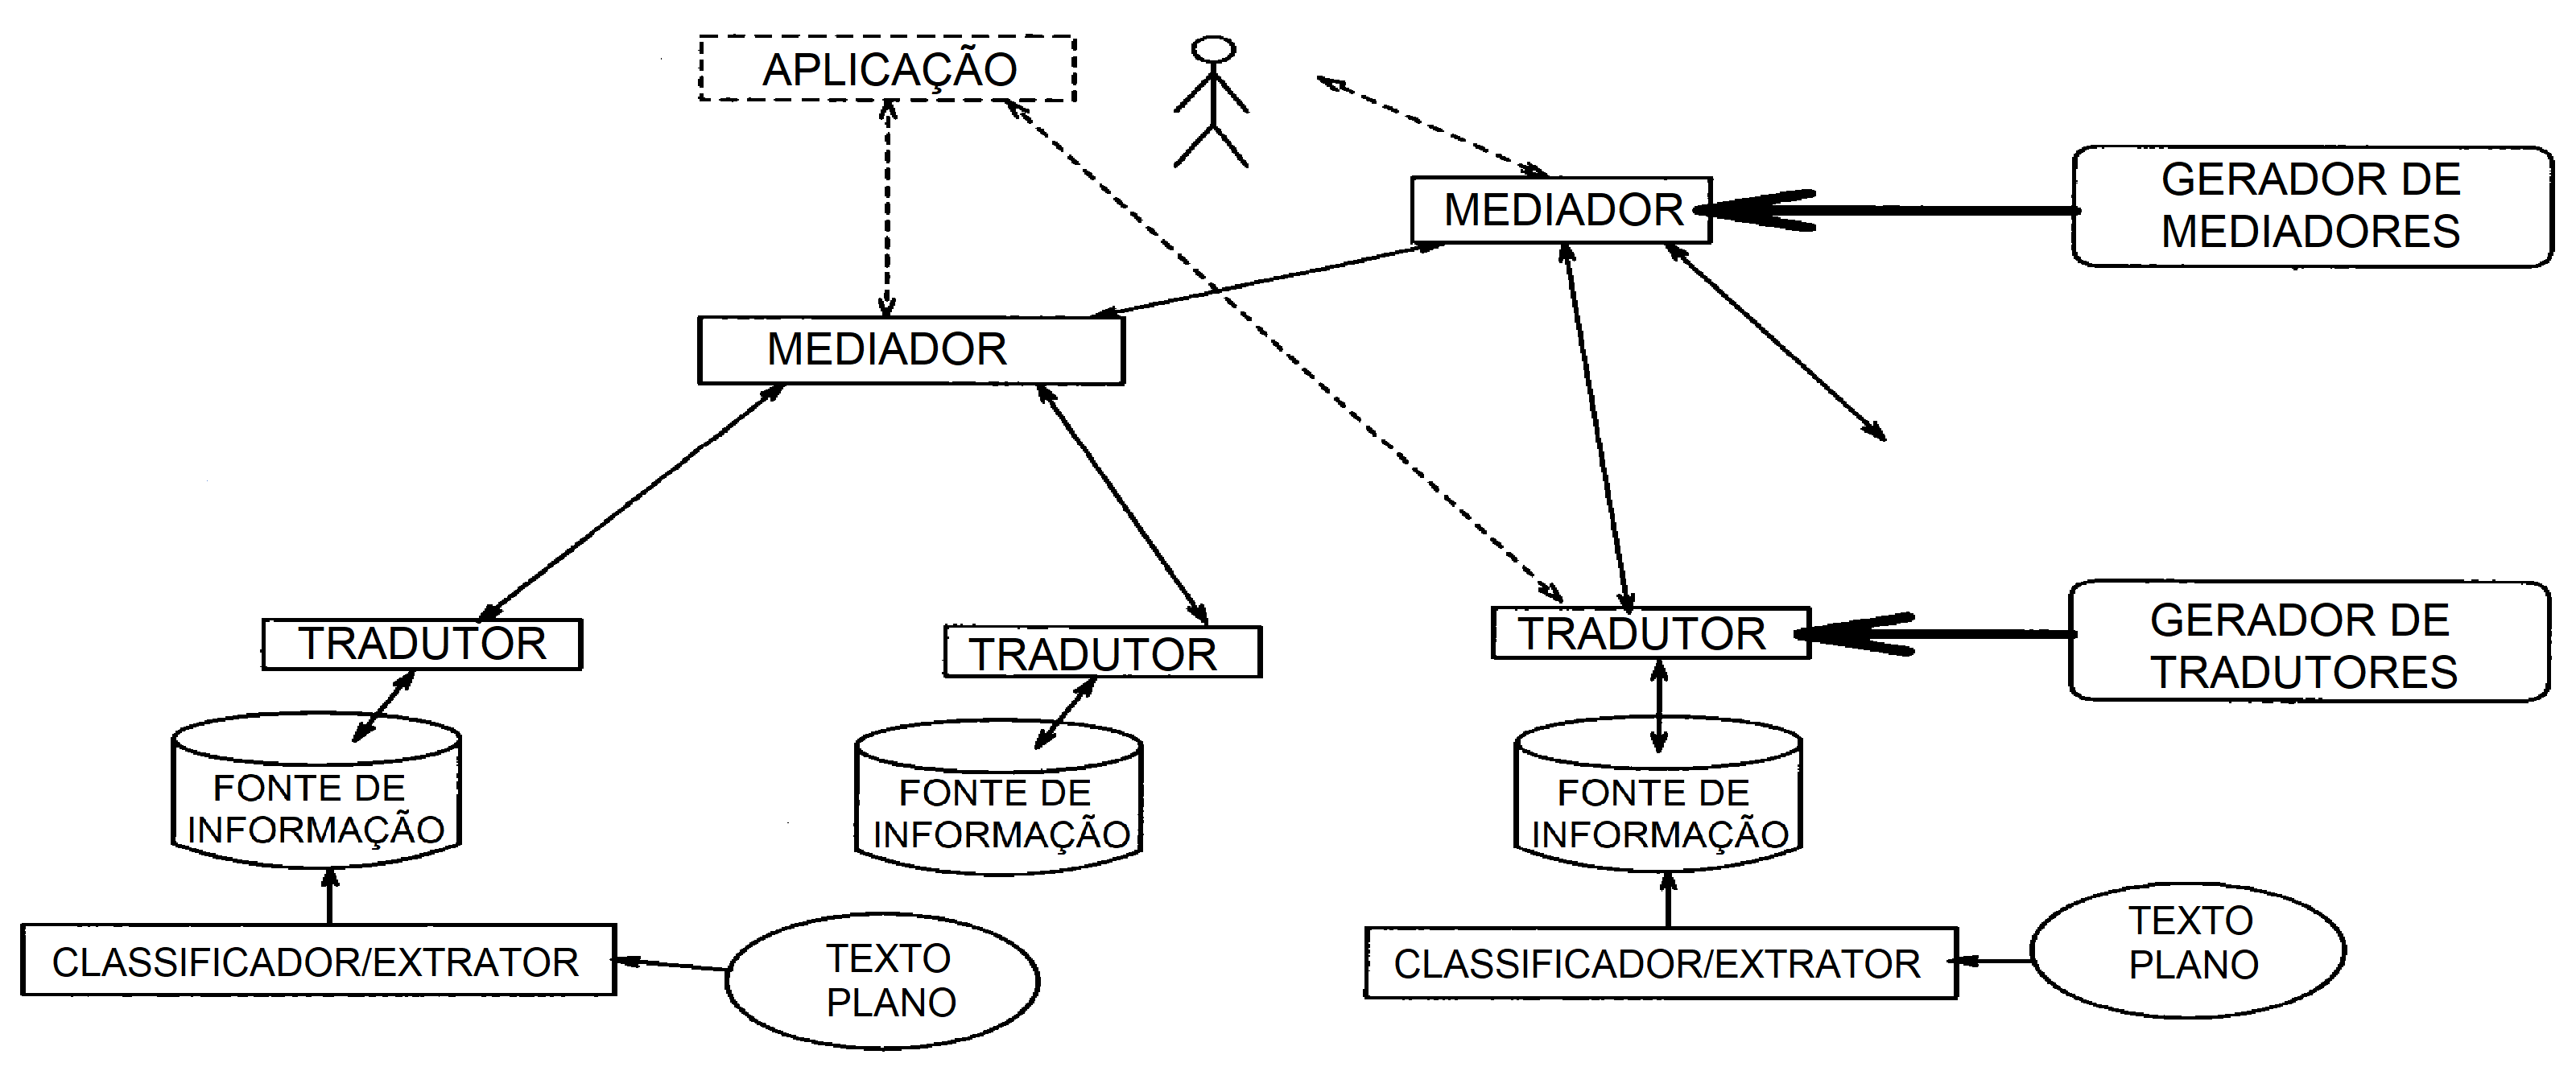
\includegraphics[width=0.3\linewidth]{figuras/TSIMMIS.png}
\caption{Abordagem virtual. Essa figura foi retirada e traduzida do artigo \cite{chawathe1994tsimmis}}
\label{fig1}
\end{figure}

\begin{figure}[!ht]
\centering
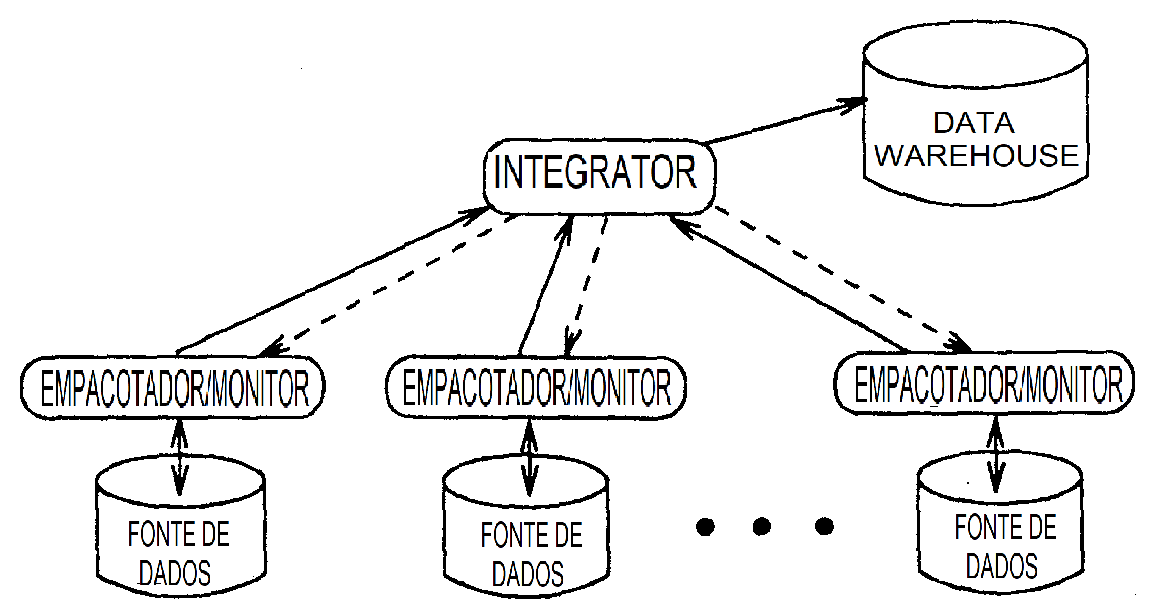
\includegraphics[width=0.3\linewidth]{figuras/DW.png}
\caption{Abordagem materializada com Data Warehouse. Essa figura foi retirada e traduzida do artigo \cite{Widom:1995:RPD:221270.221319}}
\label{fig2}
\end{figure}

No entanto, o volume de dados cresce vertiginosamente. Estima-se por exemplo que em 2020, a quantidade de dados não estruturados deverá ser em torno de 44 ZB \cite{turner2014digital}.
Dessa forma, os conjuntos de dados passaram a ter tal tamanho e estrutura que excedem as capacidades das ferramentas de programação tradicionais para coleta, armazenamento e processamento de dados em um tempo razoável e por motivos de força maior, excedem a capacidade de sua percepção por um humano \cite{miloslavskaya2014information}. Esses fatos invibializa a abordagen materializada em um cenário de Big Data, visto que o esforço para a criação de extratores, mediadores, tradutores e demais componentes supramencionados é custoso.
Os critérios que determinam a diferença entre as abordagens tradicionais (virtual e materializada) de abordagens de Big Data são os 7V: Volume, Velocidade, Variedade, Veracidade, Variabilidade, Valor e Visibilidade.

Uma tecnologia recente de Big Data que tem mostrado bons resultados são os Data Lakes.
Um data lake é um repositório centralizado que permite armazenar todos os  dados estruturados, semiestruturados e não estruturados em qualquer escala. O armazenamento é feito no formato natural dos dados \cite{laskowski2016data}. Como exemplificado na figura \ref{fig3}, a preocupação é armazenar todos os dados, sem perda, para posterior exploração.
O principal desafio dessa arquitetura é que os dados brutos são armazenados sem supervisão do conteúdo.

\begin{figure}[!ht]
\centering
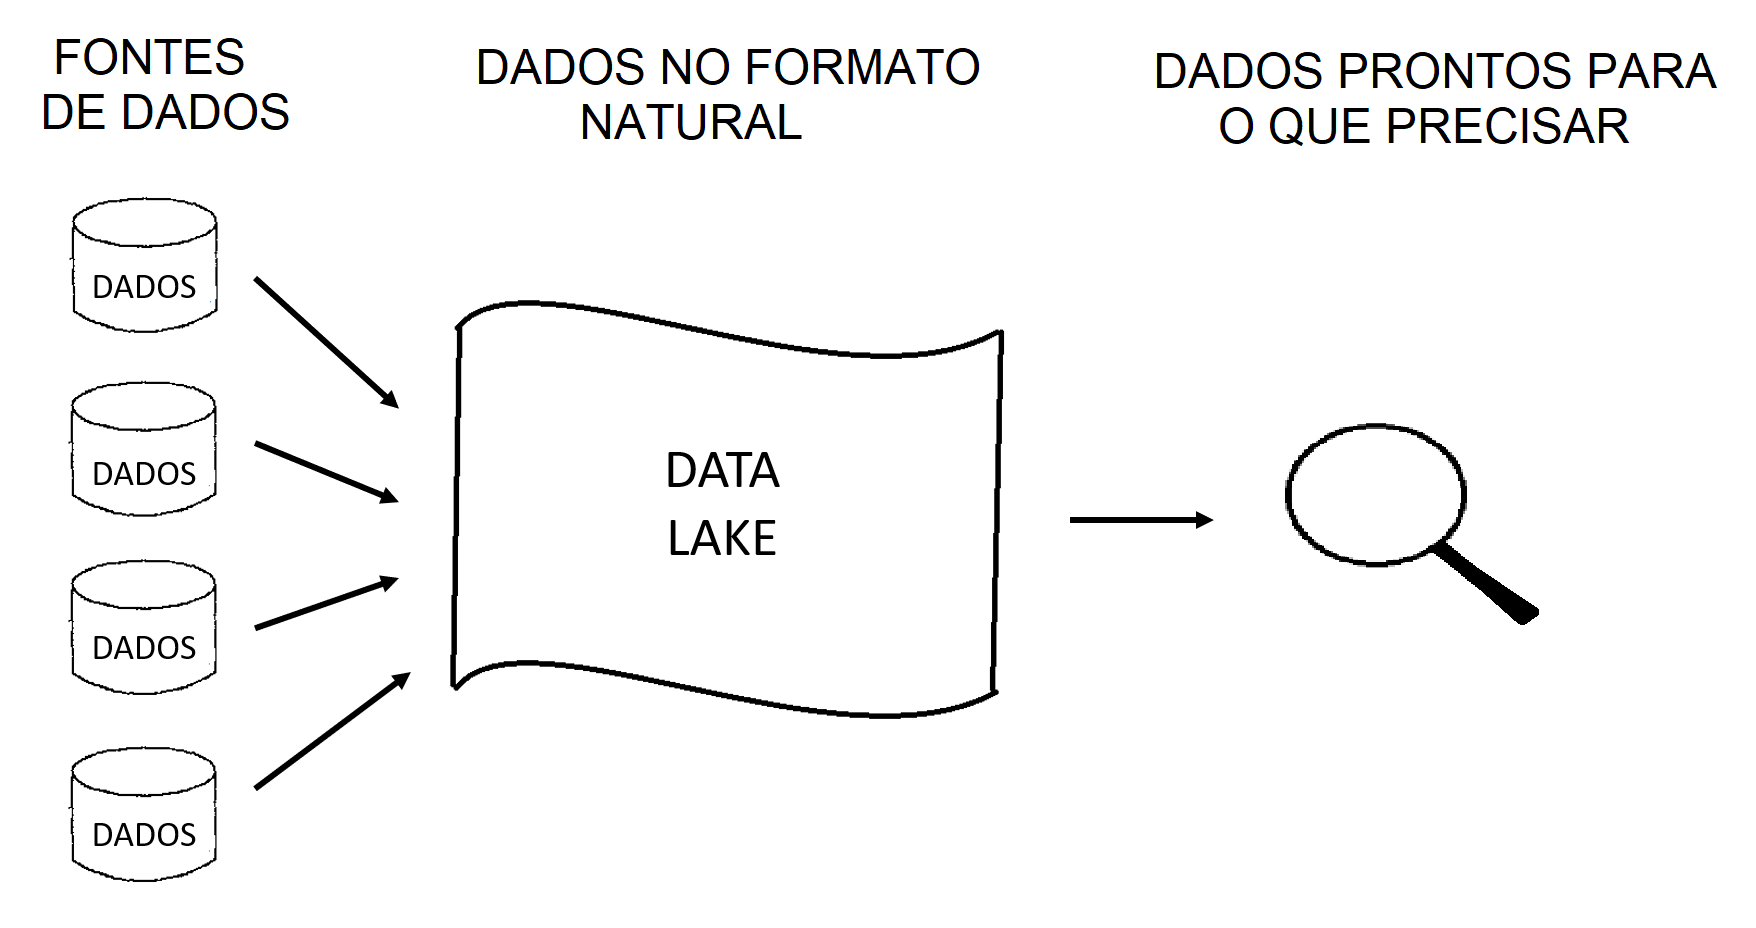
\includegraphics[width=0.3\linewidth]{figuras/DL.png}
\caption{Fluxo de um Data Lake}
\label{fig3}
\end{figure}

Um Data Lake possui as seguintes etapas:
• Injeção de dados: Os Data Lakes permitem importar qualquer quantidade de dados que possa vir em tempo real. Os dados são coletados de várias fontes e movidos para o lago de dados em seu formato original. Esse processo permite que você dimensione para dados de qualquer tamanho, economizando tempo de definição de estruturas de dados, esquemas e transformações.
• Armazenar: depois de recuperados, os dados precisam ser armazenados em um formato durável e facilmente acessível.
• Processar e analisar: nessa etapa, os dados são transformados de brutos em informações acionáveis.
• Explorar e visualizar: a etapa final é a de conversão dos resultados da análise em um formato que facilite a extração de informações e o compartilhamento.

Note que mover os dados de um armazenamento em Data Warehouse ou outras abordagens para a abordagem "armazenar tudo" de um  Data Lake é útil somente se ainda for possível extrair conhecimento de todos os dados.

existem várias ferramentas para data lake, como: Google Cloud Platform \ref{https://cloud.google.com/solutions/build-a-data-lake-on-gcp?hl=pt-br}{GCP}, \ref{https://aws.amazon.com/pt/big-data/datalakes-and-analytics/what-is-a-data-lake/?nc1=h_ls}{AWS}, \ref{https://azure.microsoft.com/pt-br/services/storage/data-lake-storage/}{Azure}.  Além de fornecer funcionalidades de Data Lake, estas ferramentas possibilitam o uso de mineração de dados, aprendizado de máquina e diversos outros recursos integrados.
Neste trabalho, utilizaremos o \ref{https://drill.apache.org/}{Apache Drill} para integrar os dados, nos valendo do conceito já apresentado de Data Lake e da integração virtualizada dos dados.


\chapter{Abordagem Proposta}

De forma geral, a abordagem proposta seguiu as seguintes etapas:
I.	Obter os dados do GAL.
II.	Armazenar os dados obtidos em seu estado bruto.
III.	Identificar as questões a serem respondidas.
IV.	Integrar os dados de forma consistente.
V.	Processar os dados.
VI.	Gerar visualização dos resultados para as questões estabelecidas.

O GAL tem suas funcionalidades limitadas por perfis de acesso, ou seja, na etapa de extração dos dados o pesquisador colaborador (especialista vinculado a FIOCRUZ) obteve somente dados provenientes dos laboratórios dessa instituição. Além disso, o sistema permite somente a exportação dos dados referentes a um período máximo de 3 meses, o que gerou vários arquivos (no formato CSV) que deveriam ser integrados. Cada um dos arquivos refere-se a solicitações ambulatoriais de pessoas suspeitas de terem contraído alguma doença, como zika. No entanto, nestas bases de dados a chave única (chave primária) é o número da solicitação e não um atributo que identifique os pacientes, dessa forma um problema a ser resolvido é a junção dos dados dos pacientes para que nas análises futuras as consultas possam ser respondidas sem duplicatas. Vale ressaltar também que muitas informações não são preenchidas corretamente, como o endereço, telefone, número da carteirinha do SUS e outros dados que poderiam facilitar a identificação dos pacientes.
Na etapa seguinte, foram armazenados 9 arquivos relacionados a zika e outros 9 relacionados a Febre Amarela. Os atributos desses arquivos seguem na \ref{tab1}. Os campos usados para a etapa de integração e processamento (requisição, paciente, data do nascimento, sexo, data dos primeiros sintomas e data da coleta) estão discriminados nas linhas de cor cinza claro. A quantidade de arquivos para cada doença deve-se ao fato da zika ter apresentado um surto entre 2015 e 2017, enquanto a febre amarela apresentou um surto de 2017 até 2018.

\begin{table}
\centering
\caption{Campos dos Arquivos Sobre Zika e Febre Amarela}
\label{tab1}
\begin{tabular}{lll}
\rowcolor[rgb]{0.502,0.502,0.502} ID & Zika                             & Febre Amarela                     \\
\rowcolor[rgb]{0.753,0.753,0.753} 1  & Requisição                       & Requisição                        \\
2                                    & Requisição Correlativo (S/N)     & Requisição Correlativo (S/N)      \\
3                                    & Regional de Cadastro             & Regional de Cadastro              \\
4                                    & Laboratório de Cadastro          & Laboratório de Cadastro           \\
5                                    & CNES Laboratório de Cadastro     & CNES Laboratório de Cadastro      \\
6                                    & Unidade Solicitante              & Unidade Solicitante               \\
7                                    & CNES Unidade Solicitante         & CNES Unidade Solicitante          \\
8                                    & Municipio do Solicitante         & Municipio do Solicitante          \\
9                                    & IBGE Município Solicitante       & IBGE Município Solicitante        \\
10                                   & Estado do Solicitante            & Estado do Solicitante             \\
11                                   & CNS do Profissional de Saúde     & CNS do Profissional de Saúde      \\
12                                   & Nome Profissional de Saúde       & Nome Profissional de Saúde        \\
13                                   & Reg. Conselho/Matrícula          & Reg. Conselho/Matrícula           \\
14                                   & Agravo da Requisição             & Agravo da Requisição              \\
15                                   & Data da Solicitação              & Data da Solicitação               \\
\rowcolor[rgb]{0.753,0.753,0.753} 16 & Data do 1º Sintomas              & Data do 1º Sintomas               \\
17                                   & Finalidade                       & Finalidade                        \\
18                                   & Descrição Finalidade             & Descrição Finalidade              \\
19                                   & Observação                       & Observação                        \\
20                                   & Núm. Notificação Sinan           & Núm. Notificação Sinan            \\
21                                   & Agravo Sinan                     & Agravo Sinan                      \\
22                                   & CID Agravo Sinan                 & CID Agravo Sinan                  \\
23                                   & Data Notificação Sinan           & Data Notificação Sinan            \\
24                                   & Unidade Notificação Sinan        & Unidade Notificação Sinan         \\
25                                   & CNES Unidade Notificação Sinan   & CNES Unidade Notificação Sinan    \\
26                                   & Município Notificação Sinan      & Município Notificação Sinan       \\
27                                   & IBGE Município Notificação SINAN & IBGE Município Notificação SINAN  \\
28                                   & Núm. Notificação Gal             & Núm. Notificação Gal              \\
29                                   & Agravo Gal                       & Agravo Gal                        \\
30                                   & CID Agravo Gal                   & CID Agravo Gal                    \\
31                                   & Data Notificação Gal             & Data Notificação Gal              \\
32                                   & Unidade Notificação Gal          & Unidade Notificação Gal           \\
33                                   & CNES Unidade Notificação Gal     & CNES Unidade Notificação Gal      \\
34                                   & Município Notificação Gal        & Município Notificação Gal         \\
35                                   & IBGE Município Notificação Gal   & IBGE Município Notificação Gal    \\
36                                   & CNS do Paciente                  & CNS do Paciente                   \\
\rowcolor[rgb]{0.753,0.753,0.753} 37 & Paciente                         & Paciente                          \\
\rowcolor[rgb]{0.753,0.753,0.753} 38 & Data de Nascimento               & Data de Nascimento                \\
39                                   & Idade                            & Idade                             \\
40                                   & Tipo Idade                       & Tipo Idade                        \\
\rowcolor[rgb]{0.753,0.753,0.753} 41 & Sexo                             & Sexo                              \\
42                                   & Idade Gestacional                & Idade Gestacional                 \\
43                                   & Nacionalidade                    & Nacionalidade                     \\
44                                   & Raça/Cor                         & Raça/Cor                          \\
45                                   & Etnia                            & Etnia                             \\
46                                   & Tipo Doc. Paciente 1             & Tipo Doc. Paciente 1              \\
47                                   & Documento Paciente 1             & Documento Paciente 1              \\
48                                   & Tipo Doc. Paciente 2             & Tipo Doc. Paciente 2              \\
49                                   & Documento Paciente 2             & Documento Paciente 2              \\
50                                   & Nome da Mãe                      & Nome da Mãe                       \\
51                                   & Endereço                         & Endereço                          \\
52                                   & Bairro                           & Bairro                            \\
53                                   & CEP de Residência                & CEP de Residência                 \\
54                                   & Municipio de Residência          & Municipio de Residência           \\
55                                   & IBGE Município de Residência     & IBGE Município de Residência      \\
56                                   & Estado de Residência             & Estado de Residência              \\
57                                   & País de Residência               & País de Residência                \\
58                                   & Zona                             & Zona                              \\
59                                   & Telefone de Contato              & Telefone de Contato               \\
60                                   & Nome da Pesquisa                 & Nome da Pesquisa                  \\
61                                   & Número Interno                   & Número Interno                    \\
62                                   & Exame                            & Exame                             \\
63                                   & Metodologia                      & Metodologia                       \\
64                                   & Exame Condicionado (S/N)         & Exame Condicionado (S/N)          \\
65                                   & Exame Restrito (S/N)             & Exame Restrito (S/N)              \\
66                                   & Exame Complementar (S/N)         & Exame Complementar (S/N)          \\
67                                   & Exame Correlativo (S/N)          & Exame Correlativo (S/N)           \\
68                                   & Data de Cadastro                 & Data de Cadastro                  \\
69                                   & Material Biológico               & Material Biológico                \\
70                                   & Localização                      & Localização                       \\
71                                   & Material Clínico                 & Material Clínico                  \\
72                                   & Amostra                          & Amostra                           \\
\rowcolor[rgb]{0.753,0.753,0.753} 73 & Data da Coleta                   & Data da Coleta                    \\
74                                   & Hora da Coleta                   & Hora da Coleta                    \\
75                                   & Usou Medicamento                 & Usou Medicamento                  \\
76                                   & Medicamento                      & Medicamento                       \\
77                                   & Data Início Sintomas             & Data Início Sintomas              \\
78                                   & Kit                              & Kit                               \\
79                                   & Fabricante                       & Fabricante                        \\
80                                   & Lote do Kit                      & Lote do Kit                       \\
81                                   & Reteste                          & Reteste                           \\
82                                   & Data do Encaminhamento           & Data do Encaminhamento            \\
83                                   & Data do Recebimento              & Data do Recebimento               \\
84                                   & Data Início do Processamento     & Data Início do Processamento      \\
85                                   & Data do Processamento            & Data do Processamento             \\
86                                   & Laboratório Responsável          & Laboratório Responsável           \\
87                                   & CNES Laboratório responsável     & CNES do Laboratório Responsável   \\
88                                   & Laboratório de Execução          & Data da Liberação                 \\
89                                   & CNES Laboratório de Execução     & Status Exame                      \\
90                                   & Data da Liberação                & 1º Campo Resultado                \\
91                                   & Status Exame                     & 2º Campo Resultado                \\
92                                   & 1º Campo Resultado               & 3º Campo Resultado                \\
93                                   & 2º Campo Resultado               & 4º Campo Resultado                \\
94                                   & 3º Campo Resultado               & 5º Campo Resultado                \\
95                                   & 4º Campo Resultado               & 6º Campo Resultado                \\
96                                   & Caso                             & Observações do Resultado          \\
97                                   & Etapa tratamento                 &                                   \\
98                                   & Tomou vacina                     &                                   \\
99                                   & Data da Última Dose              &                                   \\
100                                  & Vacina                           &                                   \\
101                                  & Tempo                            &                                   \\
102                                  & Período de Tratamento            &                                   \\
103                                  & Motivo                           &                                   \\
104                                  & Diagnóstico                      &                                   \\
\end{tabular}
\end{table}

Junto ao especialista da FIOCRUZ, foram levantadas as seguintes questões:
I.	Taxa de positividade por metodologia, considerando o tempo de coleta.
II.	Taxa de positividade por material, considerando o tempo de coleta.
III.	Relação entre materiais usados e a taxa de positividade por metodologia.
IV.	Relação, quando houver, da taxa de positividade ao ser aplicada mais de uma metodologia, considerando os tempos de coleta.
V.	Média do tempo de coleta para garantir positividade de cada metodologia e outros dados estatísticos como desvios padrão.
Nota: tempo de coleta é uma medida obtida pela diferença entre a data de coleta e a data dos primeiros sintomas.

Para integrar todos os arquivos, utilizamos o Apache Drill, que é um sistema distribuído gratuito e de código aberto, para análise ad-hoc interativa de conjuntos de dados de grande escala. Projetado para lidar com até
petabytes de dados espalhados por milhares de servidores, seu objetivo é responder a consultas ad-hoc em uma latência baixa.
A arquitetura do drill possui basicamente 3 camadas: usuário, processamento e fonte de dados.
A camada de usuário provê acesso aos dados por meio de interfaces (linha de comando, REST, API e drivers JDBC/ODBC). A camada de processamento permite plugar ou extender linguagens de consulta. Na camada dos dados, configura-se  o acesso as fontes de dado, local e/ou clusterizada. Essas fontes podem ser estruturadas, semiestruturadas ou não estruturadas. \cite{hausenblas2013apache}.
Em nosso cenário, os arquivos são textuais no formato CSV, cujo separador de atributos é o caracter ";" com campos fautantes como strings vazias. Além disso, os arquivos foram armazenados localmente. Esses fatores foram configurados em uma interface do próprio Apache Drill, para aceitar corretamente o formato e para endereçar os arquivos por meio do Sistema Padrão de Arquivos (DFS).

As tarefas de manipulação dos dados na etapa de processamento dos dados foi feita na linguagem python por meio da biblioteca \ref{https://pandas.pydata.org/}{Pandas} e o pacote \ref{http://www.numpy.org/}{NumPy}, que juntas são atualmente algumas das ferramentas mais conhecidas e poderosas em data science.
No Pandas, pudemos utilizar a estrutura de dados Dataframe para armazenar o caminho dos arquivos, a chave primária de cada tupla (número da requisição), todas as aparições dos nomes dos pacientes, seu respectivo gênero e data de nascimento. Esses dados foram processados por meio da biblioteca \ref{https://recordlinkage.readthedocs.io/en/latest/index.html}{Record Linkage Toolkit} para deduplicar os registros e identificar cada paciente.
A obtenção dos dados e a subsequente transformação em um Dataframe como descrito anteriormente foi feita por meio da biblioteca \ref{https://pydrill.readthedocs.io/en/latest/}{pydrill}, que é uma abstração para python de comandos a serem enviados ao Apache Drill, facilitando o desenvolvimento.
A identificação de duplicatas foi feita por meio de 3 etapas: limpesa dos dados, indexação e comparação.

O Dataframe resultante das etapas de processamento dos dados contém como atributos: caminho do arquivo para a tupla, chave primária do arquivo (número da requisição), código identificador (substitui as informações dos pacientes mantendo o anonimato) e tempo de coleta para a requisição da respectiva tupla.
Esse Dataframe foi salvo por meio do Apache Drill em uma view permanente.
Dessa forma é possível mapear as solicitações como pacientes únicos, ao aplicar consultas que utilizem a view e os arquivos textuais em seu formato bruto.
O fluxo de trabalho da abordagem como um todo pode ser exemplificado na figura \ref{fig4}. A tarefa de executar consultas do Apache Drill possui um fluxo interno, da própria ferramenta, que é descrito abaixo e mostrado na figura \ref{fig5}.
I. Um cliente do drill faz uma consulta. Um cliente Drill é um driver JDBC, ODBC, interface de linha de comandos ou uma API REST. Qualquer Drillbit (responsável por aceitar consultas vindas de clientes) em um cluster pode aceitar consultas. Não há conceito mestre-escravo.
II. O Drillbit analisa a consulta, otimiza-a e gera um plano de consulta distribuído que é otimizado para uma execução rápida e eficiente.
III. O Drillbit que aceita a consulta torna-se o nó Drillbit da solicitação. Ele obtém uma lista de nós Drillbit disponíveis no cluster do ZooKeeper. O Drillbit de direcionamento determina os nós apropriados para executar vários fragmentos do plano de consulta para maximizar a localidade dos dados.
IV. O Drillbit programa a execução de fragmentos de consulta em nós individuais de acordo com o plano de execução.
V. Os nós individuais concluem sua execução e retornam dados para o Drillbit de acionamento.
VI. Os resultados são encaminhados para o cliente por meio de streams.

\begin{figure}[!ht]
\centering
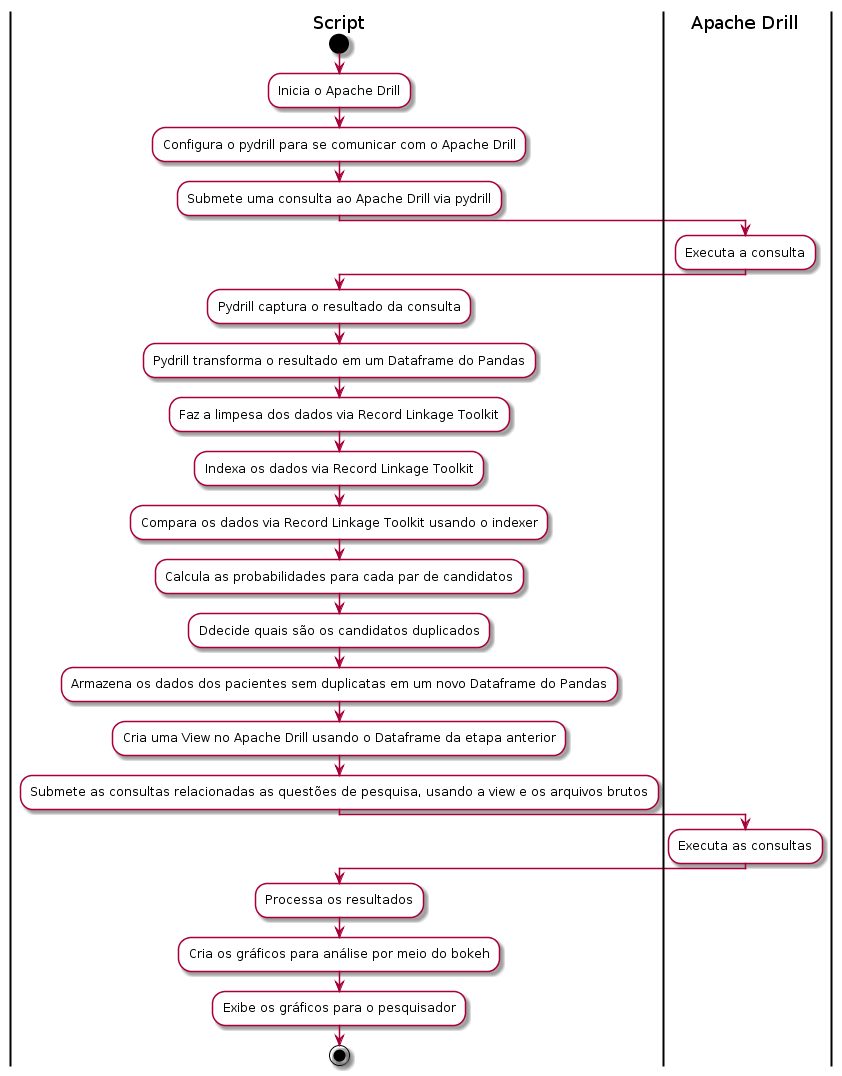
\includegraphics[width=0.3\linewidth]{figuras/wf_script.png}
\caption{Fluxo de trabalho da abordagem proposta}
\label{fig4}
\end{figure}

\begin{figure}[!ht]
\centering
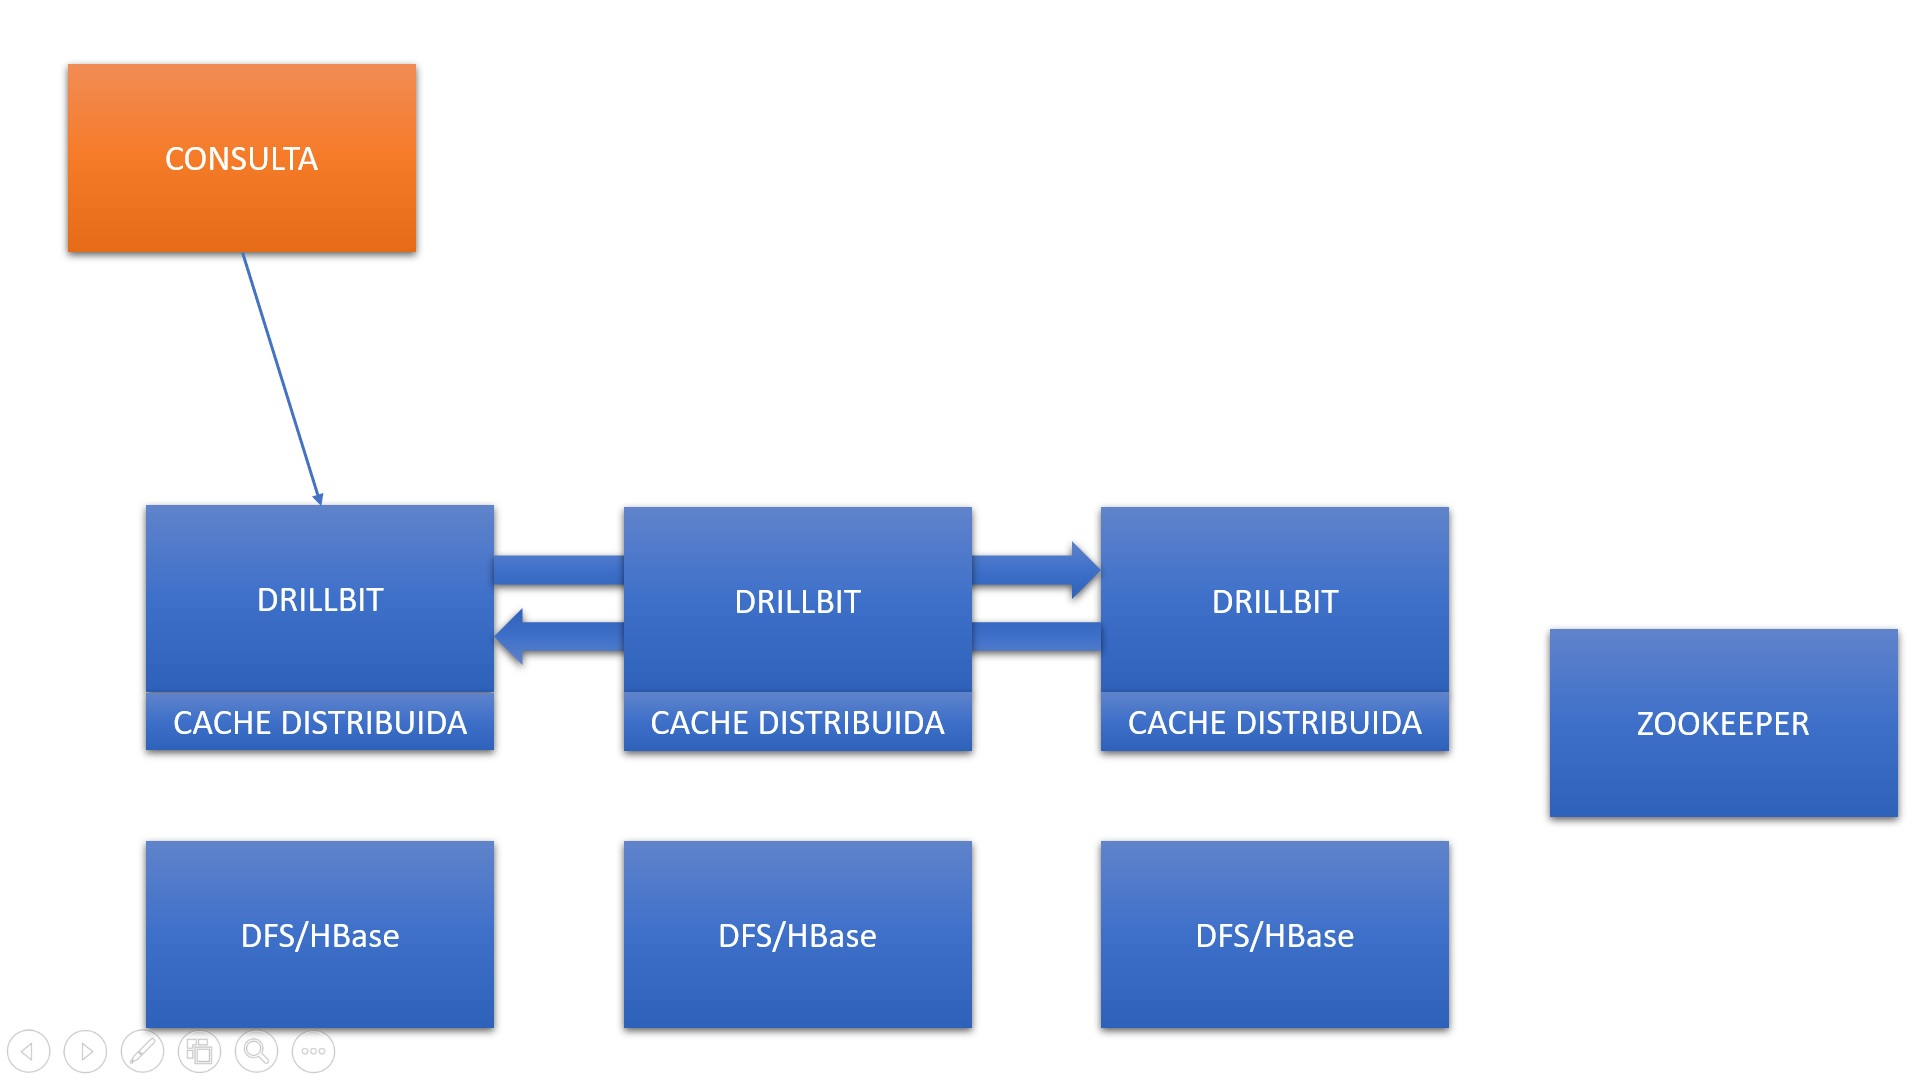
\includegraphics[width=0.3\linewidth]{figuras/wf_drill.jpg}
\caption{Fluxo interno de Consulta do Apache Drill, retirado de: https://drill.apache.org/architecture/}
\label{fig5}
\end{figure}
\chapter{Integração dos Dados}

O processo de integração de dados heterogêneos era frequentemente realizado pela abordagem virtual \cite{chawathe1994tsimmis} ou pela abordagem materializada \cite{Widom:1995:RPD:221270.221319}.
Na abordagem virtual os dados permanecem em fontes separadas e são integrados via consulta. Como pode-se observar na figura \ref{fig1}, a arquitetura dessa abordagem requer diferentes componentes. A aplicação envia consultas, que são interceptadas pelos mediadores, cuja função é direcionar para o tradutor correto, que por sua vez identifica a fonte de dados correta e efetivamente encontra a informação desejada. Caso a informação seja um dado bruto não estruturado, é requerido um classificador e extrator para a obtenção dos dados chave que representem a informação. O mediador é responsável ainda por unificar os resultados das consultas e trata-los se necessário. Os autores acreditam que pode haver um template para esses mediadores, de forma que os mesmos sejam gerados semiautomática ou automaticamente. Essa hipótese é exemplificada pelo gerador de mediadores e gerador de tradutores que devem ter esse papel.
A abordagem materializada por sua vez, possui além das fontes de dados, um empacotador que traduz as informações das fontes e um monitor que analisa a mudança nas fontes (novas fontes plugadas ou informações novas salvas em uma fonte). Em seguida os dados tratados são direcionados para o integrador que mescla os dados e os envia para o data warehouse. A arquitetura dessa abordagem pode ser analisada na \ref{fig2}. Data warehouses requerem que seus esquemas sejam definidos previamente, visto que os dados devem ser compreendidos antes da etapa de ETL (extração, transformação e carga) dos dados para o Data warehouse. As análises que são criadas unicamente no data warehouse tradicional dificultam o tratamento de dados que não estão em conformidade com um esquema bem definido, porque esses dados geralmente são descartados e perdidos.

\begin{figure}[!ht]
\centering
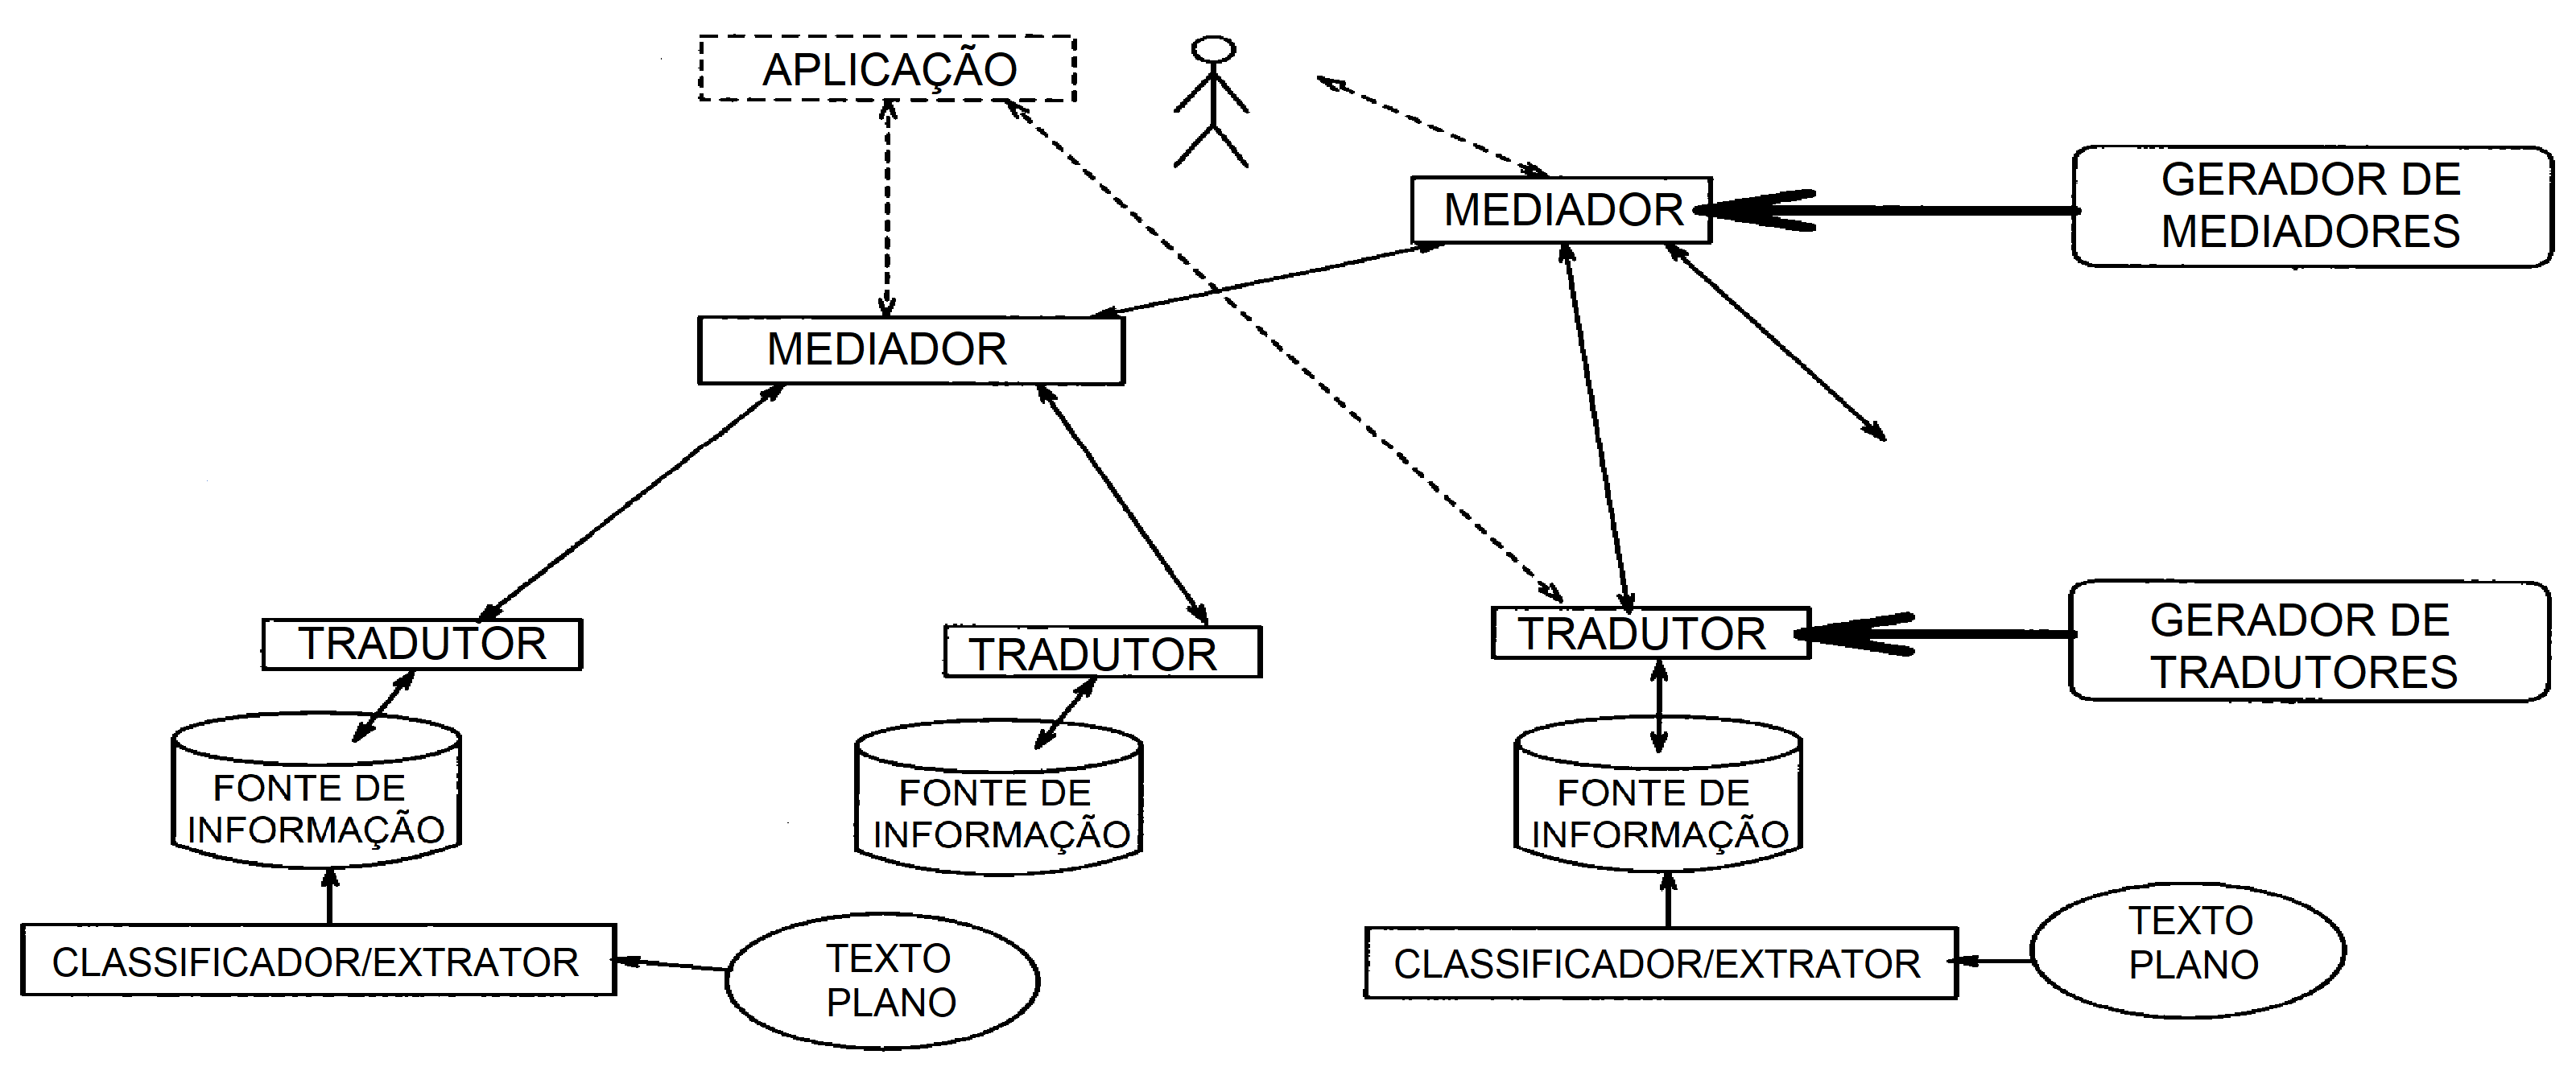
\includegraphics[width=0.3\linewidth]{figuras/TSIMMIS.png}
\caption{Abordagem virtual. Essa figura foi retirada e traduzida do artigo \cite{chawathe1994tsimmis}}
\label{fig1}
\end{figure}

\begin{figure}[!ht]
\centering
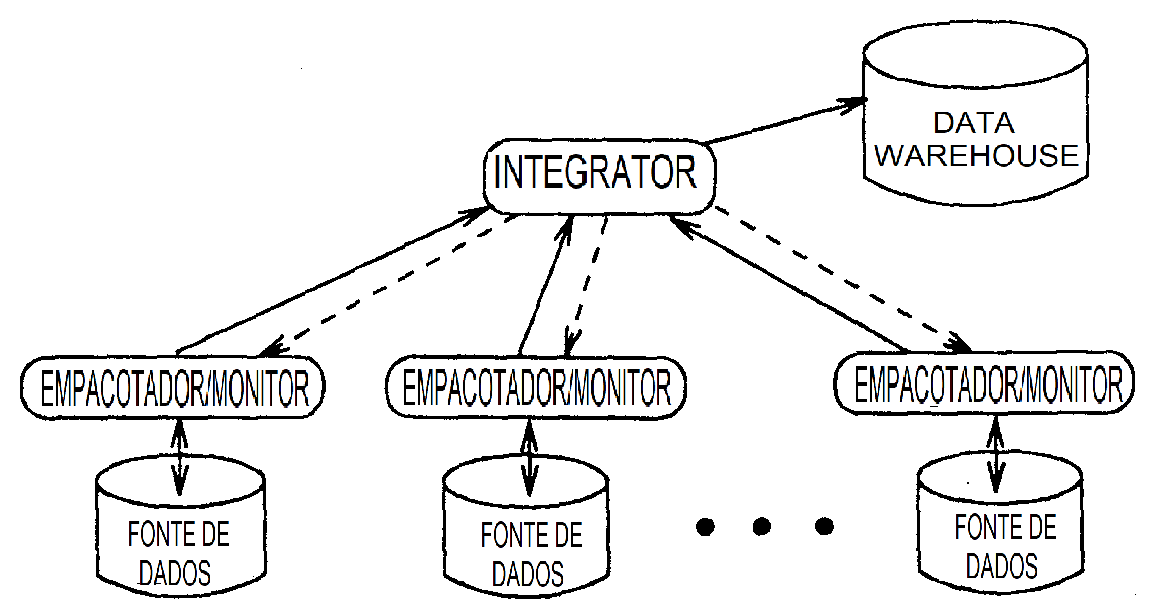
\includegraphics[width=0.3\linewidth]{figuras/DW.png}
\caption{Abordagem materializada com Data Warehouse. Essa figura foi retirada e traduzida do artigo \cite{Widom:1995:RPD:221270.221319}}
\label{fig2}
\end{figure}

No entanto, o volume de dados cresce vertiginosamente. Estima-se por exemplo que em 2020, a quantidade de dados não estruturados deverá ser em torno de 44 ZB \cite{turner2014digital}.
Dessa forma, os conjuntos de dados passaram a ter tal tamanho e estrutura que excedem as capacidades das ferramentas de programação tradicionais para coleta, armazenamento e processamento de dados em um tempo razoável e por motivos de força maior, excedem a capacidade de sua percepção por um humano \cite{miloslavskaya2014information}. Esses fatos invibializam as abordagens descritas anteriormente em um cenário de Big Data. Os critérios que determinam a diferença entre as abordagens tradicionais (virtual e materializada) de abordagens de Big Data são os 7V: Volume, Velocidade, Variedade, Veracidade, Variabilidade, Valor e Visibilidade.
Uma tecnologia recente de Big Data que tem mostrado bons resultados são os Data Lakes.
Um data lake é um repositório centralizado que permite armazenar todos os  dados estruturados, semiestruturados e não estruturados em qualquer escala. O armazenamento é feito no formato natural dos dados \cite{laskowski2016data}. Como exemplificado na figura \ref[fig3], a preocupação é armazenar todos os dados, sem perda, para posterior exploração.

\begin{figure}[!ht]
\centering
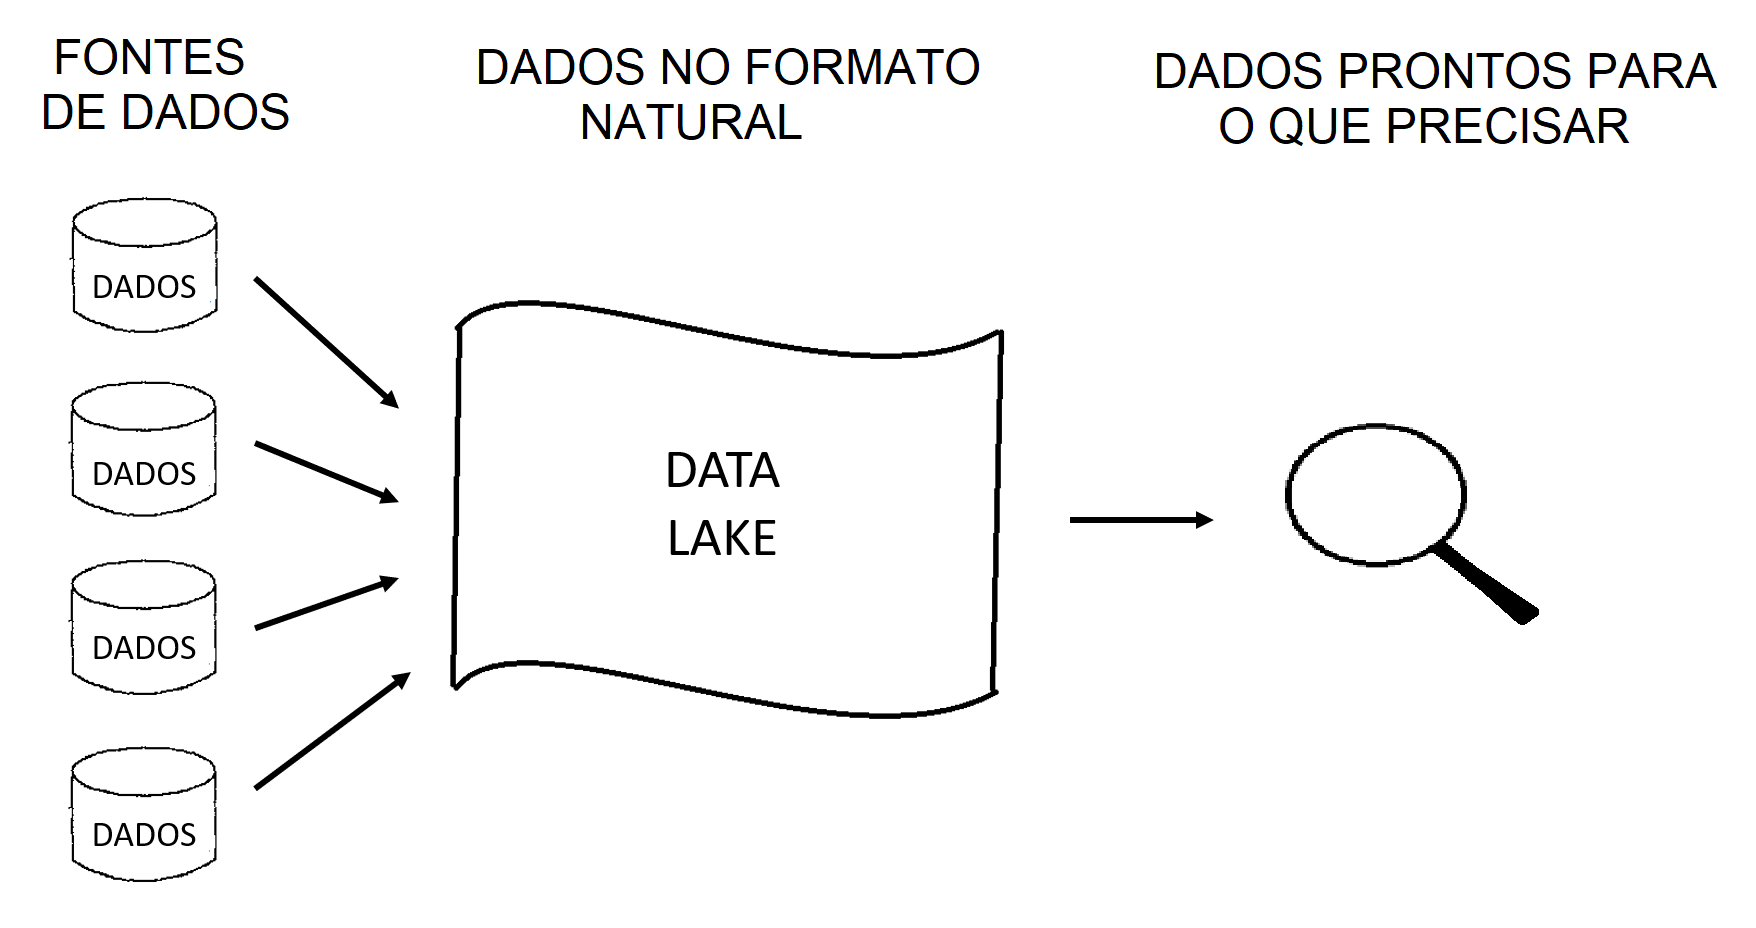
\includegraphics[width=0.3\linewidth]{figuras/DL.png}
\caption{Fluxo de um Data Lake}
\label{fig3}
\end{figure}

Um Data Lake possui as seguintes etapas:
• Injeção de dados: Os Data Lakes permitem que importar qualquer quantidade de dados que possa vir em tempo real. Os dados são coletados de várias fontes e movidos para o lago de dados em seu formato original. Esse processo permite que você dimensione para dados de qualquer tamanho, economizando tempo de definição de estruturas de dados, esquemas e transformações.
• Armazenar: depois de recuperados, os dados precisam ser armazenados em um formato durável e facilmente acessível.
• Processar e analisar: nessa etapa, os dados são transformados de brutos em informações acionáveis.
• Explorar e visualizar: a etapa final é a de conversão dos resultados da análise em um formato que facilite a extração de informações e o compartilhamento com os colegas.

Note que mover os dados de um armazenamento em Data WareHouse ou outras abordagens para a abordagem "armazenar tudo" de um  Data Lake é útil somente se ainda for possível extrair conhecimento de todos os dados.
Vale ressaltar que o principal desafio de uma arquitetura de Data Lake é que os dados brutos são armazenados sem supervisão do conteúdo.
existem várias ferramentas para data lake, como: Google Cloud Platform \ref{https://cloud.google.com/solutions/build-a-data-lake-on-gcp?hl=pt-br}{GCP}, \ref{https://aws.amazon.com/pt/big-data/datalakes-and-analytics/what-is-a-data-lake/?nc1=h_ls}{AWS}, \ref{https://azure.microsoft.com/pt-br/services/storage/data-lake-storage/}{Azure}.  Além de fornecer funcionalidades de Data Lake, estas ferramentas possibilitam o uso de mineração de dados, aprendizado de máquina e diversos outros recursos integrados.
Neste trabalho, utilizaremos o \ref{https://drill.apache.org/}{Apache Drill} para integrar os dados, nos valendo do conceito já apresentado de Data Lake.
O Apache Drill é um sistema distribuído gratuito e de código aberto, para análise ad-hoc interativa de conjuntos de dados de grande escala. Projetado para lidar com até
petabytes de dados espalhados por milhares de servidores, seu objetivo é responder a consultas ad-hoc em uma latência baixa.
A arquitetura do drill possui basicamente 3 camadas: usuário, processamento e fonte de dados.
A camada de usuário provê acesso aos dados por meio de interfaces (linha de comando, REST, API e drivers JDBC/ODBC). A camada de processamento permite plugar ou extender linguagens de consulta. Na camada dos dados, configura-se  o acesso as fontes de dado, local e/ou clusterizada. Essas fontes podem ser estruturadas, semiestruturadas ou não estruturadas. \cite{hausenblas2013apache}.
\chapter{Visualização dos Dados}

\chapter{Conclusão}

\section{Trabalhos Futuros}
	(1) Integração com outros Portais do SUS em http://www2.datasus.gov.br/DATASUS/index.php?area=04

% --- -----------------------------------------------------------------
% --- Referencias Bibliograficas. (Obrigatorio)
% --- -----------------------------------------------------------------
\cleardoublepage
\bibliographystyle{acm-2} % abbrv - abnt-num
%\bibliographystyle{uff-ic}
\bibliography{bibliografia} % arquivo fonte com a bibilografia

% --- -----------------------------------------------------------------
% --- Apendice.(Opcional)
% --- -----------------------------------------------------------------
\cleardoublepage
\appendix
\chapter{<T\'ITULO DO AP\^ENDICE>}
\label{apend}

% Este ap�ndice apresenta informa��es complementares.

Elemento opcional. O(s) ap�ndice(s) s�o identificados por letras mai�sculas consecutivas, travess�o e pelos respectivos t�tulos. Excepcionalmente utilizam-se letras mai�sculas dobradas, na identifica��o, quando esgotadas as 23 letras do alfabeto (ABNT, 2005).


\end{document}

